% 2023年北京高考数学第15题解析图2：参数a的分段函数图象
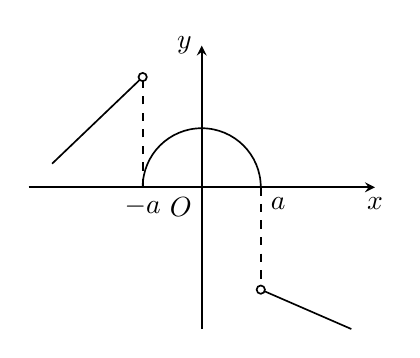
\begin{tikzpicture}[>=stealth,line width=0.6pt,font=\normalsize]
  \draw[->] (-2.2,0) -- (2.2,0) node[below] {$x$};
  \draw[->] (0,-1.8) -- (0,1.8) node[left] {$y$};
  \node[below left] at (0,0) {$O$};

  % 半圆
  \draw (0.75,0) arc[start angle=0,end angle=180,radius=0.75];
  \node[below] at (-0.75,0) {$-a$};
  \node[below right] at (0.75,0) {$a$};

  % 左侧分支
  \draw[dashed] (-0.75,0) -- (-0.75,1.4);
  \draw (-1.9,0.3) -- (-0.75,1.4);
  \draw[fill=white] (-0.75,1.4) circle (1.5pt);

  % 右侧分支
  \draw[dashed] (0.75,0) -- (0.75,-1.3);
  \draw (0.75,-1.3) -- (1.9,-1.8);
  \draw[fill=white] (0.75,-1.3) circle (1.5pt);
\end{tikzpicture}
